\section{Introduction}
\label{sec:introduction}

\todo{Axel and Regis write this...}

Gamma-ray astronomy is a rather young field of research. By detecting and
reconstructing arrival direction, time and energy of primary cosmic gamma-rays
The gamma-ray sky is either observed by ground based instruments, driven by
experiments with proprietary software often based on ROOT, because of the
particle physics background. Such as HESS, Veritas or Magic.

The Cherenkov Telescope Array (CTA) will be operated as an open observatory for
the first time. Thus there is a need for open analysis software as well.

Moreover, the operation of CTA as an observatory introduces the necessity of
sharing its data publicly. The data-reduction workflow of different IACTs of
the current generation is remarkably similar, resulting in a \textit{high} data
level that can be finally used to derive scientific results (, spectra, sky
maps, light curves). The information in this high data level is independent on
the data reduction, and eventually of the detection technique. This implies,
for example, that data from IACT and WCD can be represented within the same
model. The efforts to prototype the future CTA data model and to convert
current IACT data in a format usable with the newly-available science tools
converged in the so-called \textit{Data Format for Gamma-ray Astronomy}
initiative~\citep{gadf_proc, gadf_universe}, abbreviated in
\texttt{gamma-astro-data-format} (GADF). The latter proposes prototypical
specifications to produce files based on the flexible image transport system
(FITS) format~\citep{fits} encapsulating this high-level information. This is
realized by storing a list of gamma-like events with their measured quantites
(energy, direction, arrival time) and a parametrisation of the response of the
system (see Sec.~\ref{ssec:gammapy-data} and Sec.~\ref{ssec:gammapy-irf} for
more information).

In recent years Python \footnote{\PythonUrl} has established as one of the
standard programming  languages for astronomy \footnote{Citation missing} as
well as data sciences in  general \footnote{Citation missing}. The success is
mostly attributed to the simple and easy to learn syntax, the ability to act as
a "glue" language between different programming languages, the rich eco-system
of packages and the open and supportive community.

Astronomical data analysis software written in Python existed since 2000. e.g.,
sherpa~\citep{sherpa-2011, sherpa-2009}, or for gamma-ray even PyFACT
~\citep{pyfact}.

The short-term success of Pythion lead to a prolifaration of packages, until
\astropy~\citep{astropy} was created in 2012. Astropy is and Gammapy is a
Python package for gamma-ray astronomy.

% TODO: describe Context

% TODO: describe goals

TODO: Figure 1: Data -> Gammapy -> Spectra etc with some details

Basic idea: build on Numpy and Astropy, use Python stack

TODO: Figure 2: Gammapy software stack

Here's a list of references I'd like to cite ... to be incorporated into the
main text somewhere:

\begin{itemize}
	\item Gammapy webpage\footnote{\GammapyUrl}
	\item Naima\footnote{\NaimaUrl}~\citep{Naima}
	\item Gammapy use in science publications:~\citep{Owen2015}, SNR shell, HGPS
\end{itemize}

* Gammapy – A Python package for gamma-ray astronomy
* Gammapy – A prototype for the CTA science tools
* Astropy: A community Python package for astronomy
* THE ASTROPY PROJECT: BUILDING AN INCLUSIVE, OPEN-SCIENCE PROJECT AND STATUS
OF THE V2.0 CORE PACKAGE * GammaLib and ctools * Fermipy proceedings * SunPy:
Python for Solar Physics. An implementation for local correlation tracking *

\begin{figure}[t]
	\centering
	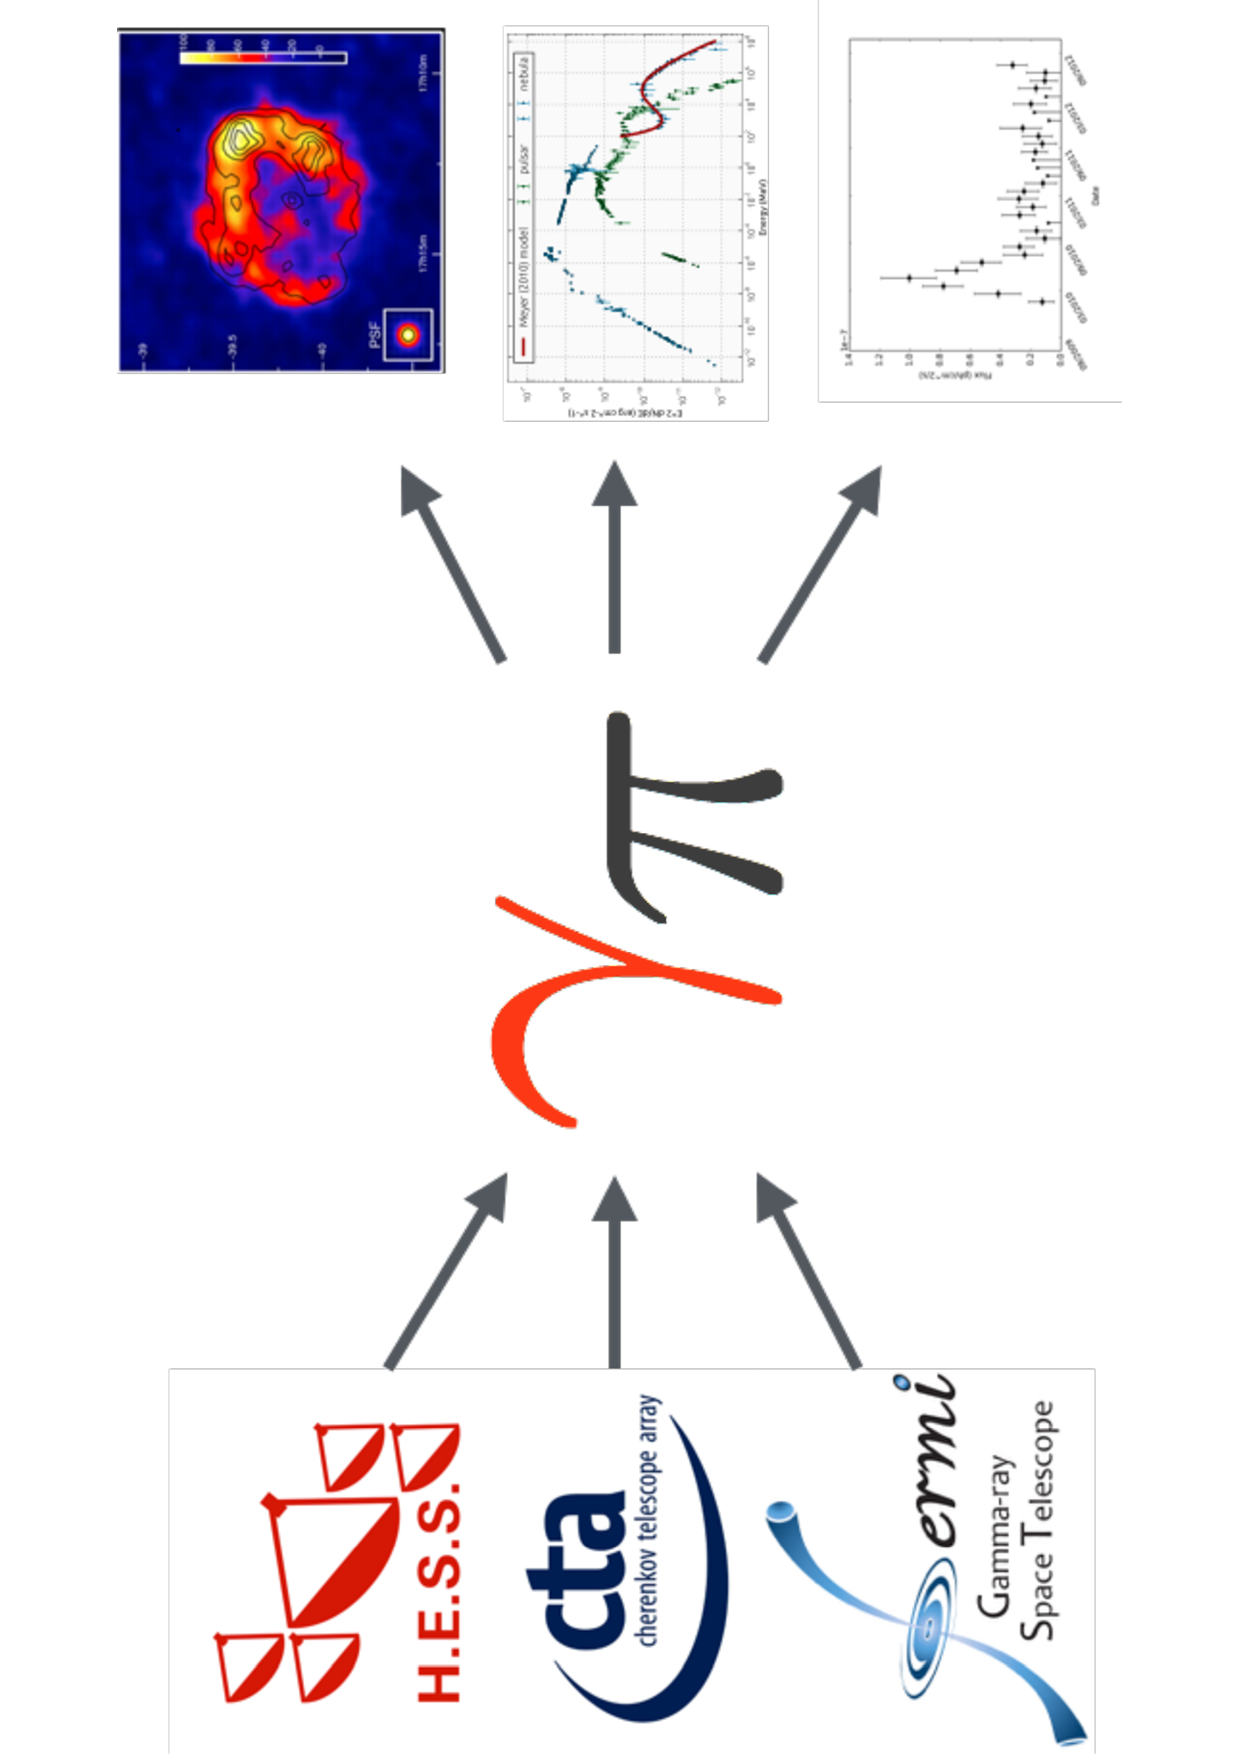
\includegraphics[height=0.5\textwidth,
		angle=270]{static/gammapy-big-picture} \caption{ Gammapy is a Python package
		for high-level gamma-ray data analysis. Using event lists, exposures and point
		spread functions as input you can use it to generate science results such as
		images, spectra, light curves or source catalogs. So far it has been used to
		simulate and analyse H.E.S.S., CTA and \textit{Fermi}-LAT data, hopefully it
		will also be applied to e.g., VERITAS, MAGIC or HAWC data in the future. }
	\label{fig:big-picture}

\end{figure}

\begin{figure}[t]
	\centering
	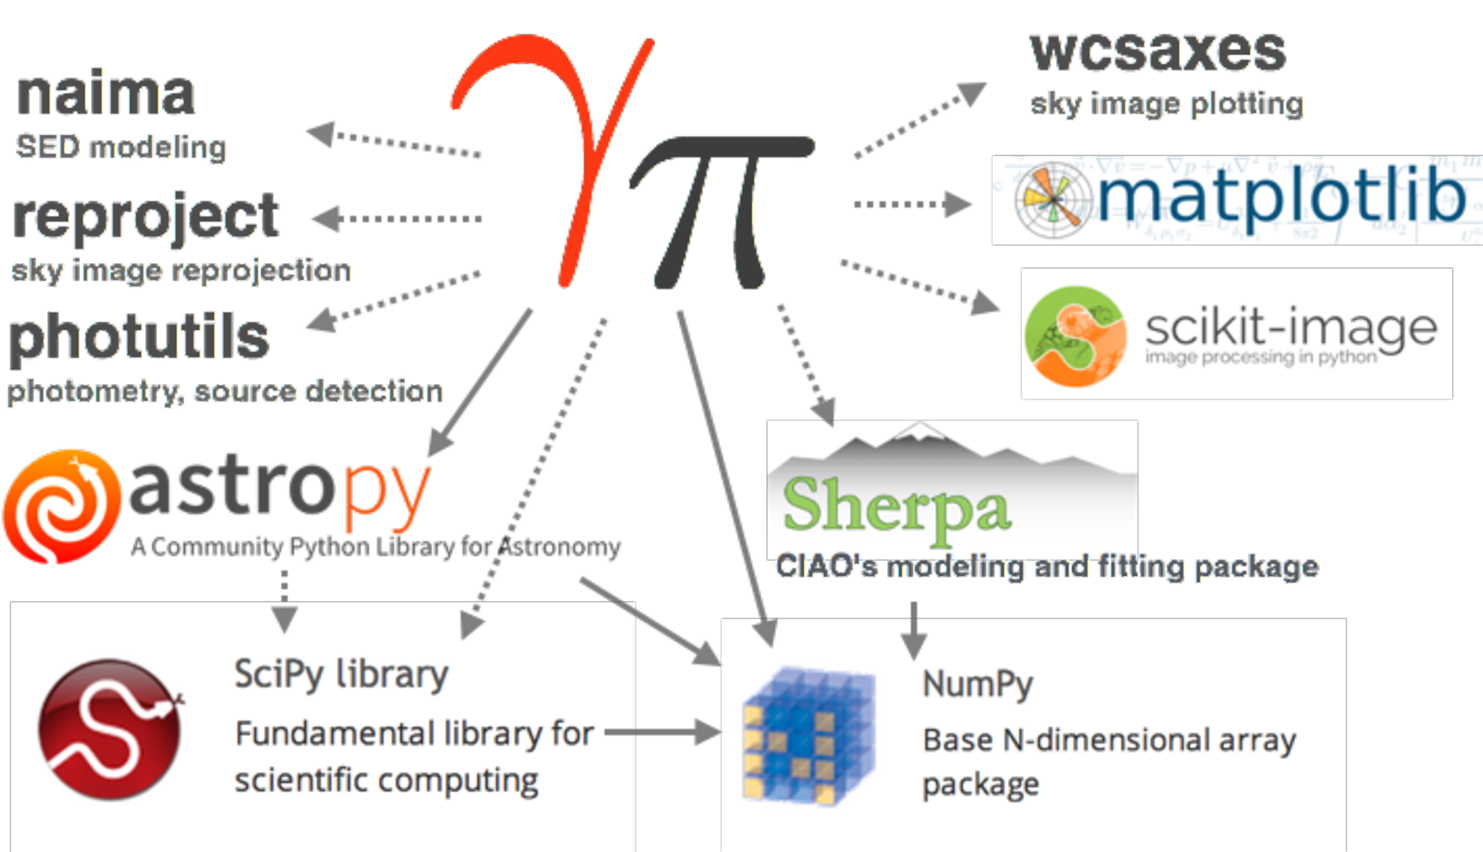
\includegraphics[width=0.5\textwidth]{static/gammapy-dependencies}
	\caption{
		The Gammapy stack. Required dependencies Numpy and Astropy are illustrated with
		solid arrows, optional dependencies (the rest) with dashed arrows. }
	\label{fig:dependencies}

\end{figure}

